\documentclass[a4paper,twoside,11pt]{book}


% Import packages
\usepackage[utf8]{inputenc}
\usepackage{kotex}
\usepackage{titlesec}
\usepackage{color}
\usepackage{physics}
\usepackage[a4paper,margin=1in]{geometry}
\usepackage{graphicx}
\usepackage{wrapfig}
\usepackage{fancyhdr}
\usepackage{setspace}
\usepackage{xcolor}
\usepackage{mdframed}
\usepackage{amsmath}


% Section for boxed highlight text
\newmdenv[
  backgroundcolor=gray!20,
  skipabove=\topsep,
  skipbelow=\topsep,
]{keypoint}

\makeatletter
\let\orig@keypoint=\keypoint
\def\keypoint{
  \@ifnextchar[{\keypoint@opt}{\orig@keypoint}
}
\def\keypoint@opt[#1]{
  \orig@keypoint[frametitle={#1}]
}
\makeatother


% Custom placeholder command with counter to keep track
\newcounter{placeholder}
\newcommand{\placeholder}{\stepcounter{placeholder}\textcolor{red}{PLACEHOLDER \theplaceholder}}


% Set graphics import path
\graphicspath{ {./images/} }


% Set various spacing
\onehalfspacing

\setlength{\textfloatsep}{1pt}
\setlength{\intextsep}{1pt}
\setlength{\belowcaptionskip}{3pt}
\setlength{\headheight}{15pt}
\setlength{\parskip}{1pt}
\setlength{\dbltextfloatsep}{1pt}
\setlength{\dblfloatsep}{1pt}
\setlength{\floatsep}{1pt}


% Set text to Korean
\renewcommand{\contentsname}{목차}
\renewcommand{\thechapter}{\arabic{chapter}장}
\renewcommand{\chaptername}{제}
\renewcommand{\thesection}{\arabic{chapter}.\arabic{section}}
\renewcommand{\figurename}{그림}
\renewcommand{\thefigure}{\arabic{chapter}.\arabic{figure}}


% maketitle content
\title{Project Principia}
\author{하나고등학교 유진일
\and 하나고등학교 이윤규}
\date{2019년 5월}


% Page header and footer
\fancypagestyle{plain}{
    \fancyhf{}
    \renewcommand{\headrulewidth}{1pt}
    \renewcommand{\footrulewidth}{0pt}
    \fancyhead[LE,RO]{\leftmark}
    \fancyhead[RE,LO]{\rightmark}
    \fancyfoot[LE,RO]{\thepage}
    \fancyfoot[RE,LO]{Project Principia}
}

\pagestyle{plain}
    

% Begin main document
\begin{document}
\maketitle

\pagenumbering{roman}

\tableofcontents

\chapter[\quad 벡터]{벡터}

\pagenumbering{arabic}

\section{벡터의 성질}

\subsection{기본 정의}

\begin{wrapfigure}[4]{O}{0.35\textwidth}
  \centering
  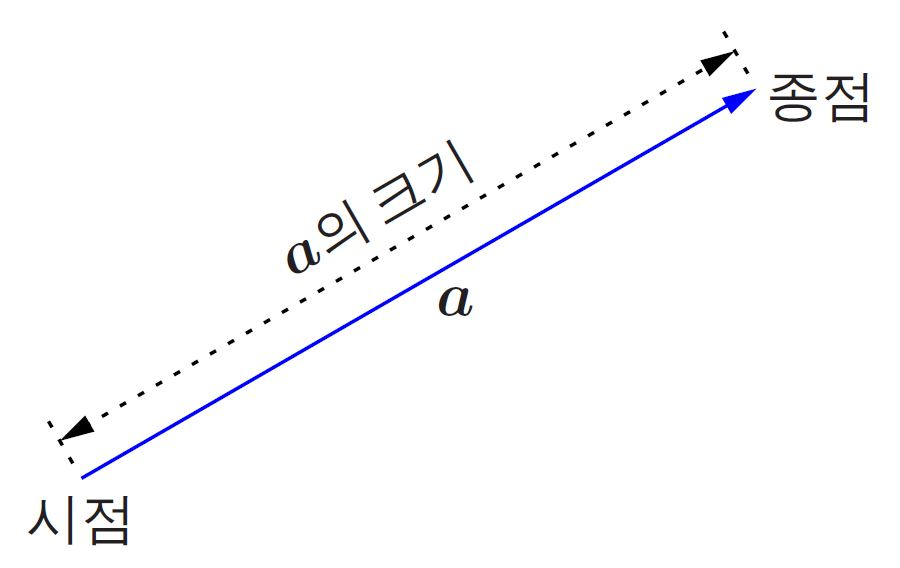
\includegraphics[width=0.34\textwidth]{images/fig1-1}
  \caption{화살표에 의한 벡터}
  \label{fig:arrowvector}
\end{wrapfigure}

스칼라(scalar)는 하나의 숫자인 크기와 그 단위만으로 나타낼 수 있는 물리량이다.
\begin{description}\item[$\bullet$]{스칼라의 예:} 온도 $T$, 밀도 $\rho$, 시간 $t$ \end{description}
벡터(vector)는 크기와 함께 공간속에서의 방향까지 지정하는 물리량이다.
\begin{description}\item[$\bullet$]{벡터의 예:} 힘 $\va{F}$, 가속도 $\va{a}$, 속도 $\va{v}$ \end{description}

벡터는 스칼라와 구분하여 위의 예와 같이 문자 위에 화살표를 표시하거나 다음과 같이 굵은 글씨(볼드체)로 표기한다.

\begin{keypoint}[벡터의 표기법]
  모든 벡터는 다음과 같이 어떠한 문자 위헤 화살표를 배치하거나, 굵은 문자로 나타내도록 한다.
  $$\va{a}, \vb{v}, \va{v}, \vb{a}$$
\end{keypoint}


공간 상에 벡터를 표시할 때에는 그림 \ref{fig:arrowvector}와 같이 화살표로 나타낸다. 화살표의 길이는 벡터의 크기를 나타내고 벡터의 방향은 화살표가 가리키는 방향이 된다.

벡터의 크기는 절댓값 기호를 이용하여 나타내며, 간단하게 본래 벡터를 나타내는 기호에서 화살표를 제거하거나 혹은 볼드체의 본래의 글자체로 표기하여 나타내기도 한다.
$$\abs{\va{a}} = \abs{a} = a $$
만약 n-공간의 어떠한 벡터를 $\vb{a} = (a_1, a_2, a_3, a_4, \cdots, a_n)$으로 나타냈다면, 벡터 $\vb{a}$의 크기는 아래와 같다.

\begin{keypoint}[벡터의 표기법]
  n-공간의 벡터 $\vb{a} = (a_1, a_2, a_3, \cdots, a_n)$에 대하여 벡터의 크기는 다음과 같이 주어진다.
  $$\abs{\vb{a}} = \sqrt{{a_1}^2 + {a_2}^2 + {a_3}^2 + \cdots + {a_n}^2 }$$
\end{keypoint}

이러한 벡터 중, 크기가 1인 벡터를 특별히 단위 벡터라 부르며, 벡터 $\vb{a}$와 평행한 단위 벡터를 $\vu{a}$ 또는 $\vb{e}_a$로 나타내기로 약속한다.

벡터 $\vb{a}$에 스칼라 $\lambda$를 곱한 양 $\lambda\vb{a}$도 벡터이다. 그 크기는 $\abs{\lambda}a$이며, 방향은 $\vb{a}$와 평행하되 $\lambda>0$인 경우에는 $\vb{a}$와 같은 방향을 가르키고, $\lambda<0$의 경우는 $\vb{a}$의 반대방향을 가르킨다.

\subsection{벡터의 덧셈과 뺄셈}

벡터의 덧셈과 뺄셈은 그림 \ref{fig:addsubvector}와 같이 계산한다.

\begin{wrapfigure}{I}{0.35\textwidth}
  \centering
  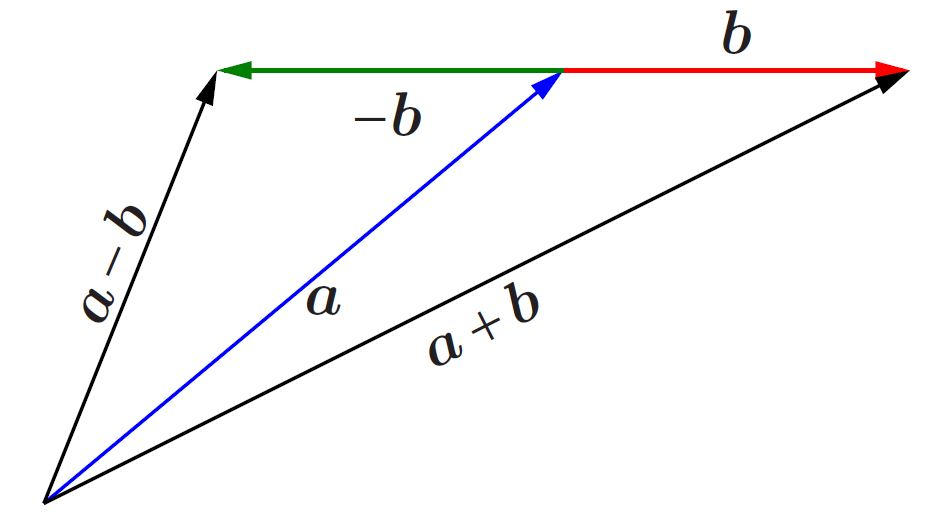
\includegraphics[width=0.34\textwidth]{images/fig1-2}
  \caption{벡터의 덧셈과 뺄셈}
  \label{fig:addsubvector}
\end{wrapfigure}

$\vb{a} + \vb{b}$는 $\vb{a}$의 화살표 끝과 $\vb{b}$의 화살표 시작점을 일치 시켰을 때 그릴 수 있는 삼각형의 나머지 한 변에 평행하고 방향은 $\vb{a}$의 시점으로부터 $\vb{b}$의 종점을 향한다. $\vb{a} - \vb{b}$는 $\vb{a} + (-\vb{b})$와 동일하며 따라서 $\vb{a}$와 $-\vb{b}$로 그릴 수 있는 삼각형의 나머지 한변과 평행하고 방향은 $\vb{a}$의 시점에서 $-\vb{b}$의 종점을 향한다.

벡터의 덧셈과 뺄셈은 교환 법칙과 결합 법칙이 성립한다.
$$\vb{a} + \vb{b} = \vb{b} +\vb{a}, \quad \vb{a} + (\vb{b} + \vb{c}) = (\vb{a} + \vb{b}) + \vb{c}$$

\subsection{기저 벡터}

평면 상의 임의의 벡터는 두 개의 서로 다른 벡터의 선형 결합으로 모두 나타낼 수 있다. 여기서 벡터들의 선형 결합이란 상수 $\alpha$, $\beta$와 벡터 $\vb{a}$, $\vb{b}$에 대하여 $\alpha\vb{a} + \beta\vb{b}$의 꼴을 의미하며, 마찬가지로 3차원 공간에서는 3개의 서로 다른 벡터의 선형 결합으로 모든 벡터를 나타낼 수 있다. 이 벡터들을 기저 벡터(basis)라고 부른다.

\begin{wrapfigure}{I}{0.35\textwidth}
  \centering
  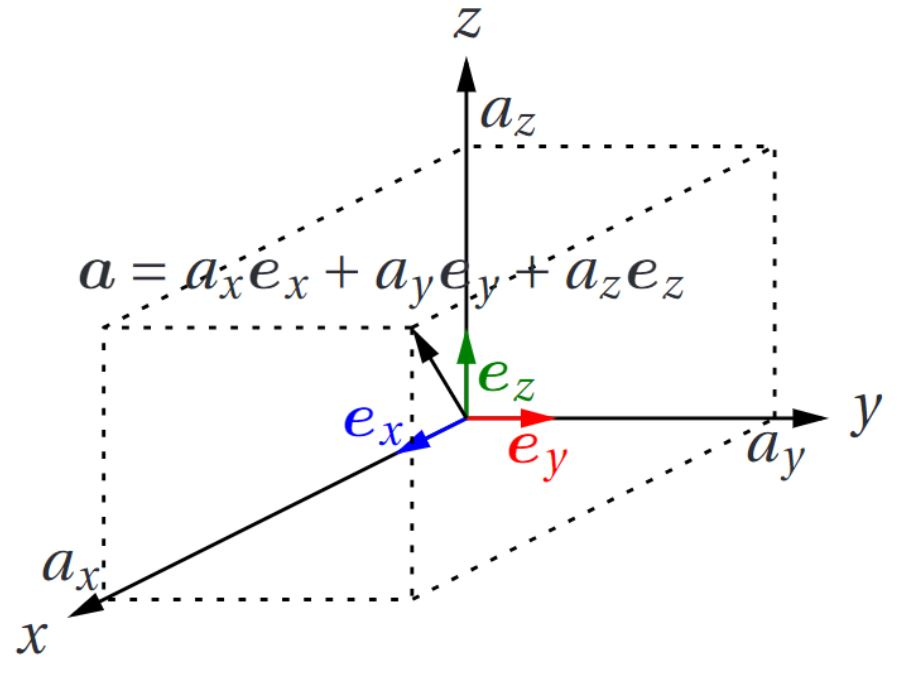
\includegraphics[width=0.34\textwidth]{images/fig1-3}
  \caption{데카르트 좌표계의 기저 벡터}
  \label{fig:cartesianbasis}
\end{wrapfigure}

기저 벡터들은 서로 평행하지만 않으면 얼마든지 원하는 대로 선택할 수 있다. 그러나 일반적으로는 데카르트 좌표계(Cartesian coordinate system)\footnote{일반적으로 많이 쓰이는 xyz축에 의해 나타내어지는 삼차원 직교 좌표계의 이름이다.}에서 그림 \ref{fig:cartesianbasis}과 같이 각 축에 평행한 단위 벡터를 기저 벡터로 선택하고 이들은 주로 다음과 같은 기호로 나타낸다.
$$\vb{e}_x, \vb{e}_y, \vb{e}_z \quad \textrm{또는} \quad \vu{i}, \vu{j}, \vu{k}$$
이들은 \textbf{기본 단위 벡터}라고 불리며, 단위 벡터이므로 크기가 모두 1로 같고 서로 수직이다.
$$\abs{\vb{e}_i} = 1 \ (i=x,y,z), \quad \vb{e}_i \perp \vb{e}_j \ (i \neq j)$$
그림 \ref{fig:cartesianbasis}처럼 임의의 벡터는 기본 단위 벡터의 이들의 선형결합으로 나타낼 수 있다.
$$\vb{a} = a_x \vb{e}_x + a_y \vb{e}_y + a_z \vb{e}_z = \sum^{x,y,z}_{i}a_i \vb{e_i}$$
이때 $a_x, a_y, a_z$를 각각 $\va{a}$의 $x$성분, $y$성분, $z$성분이라 하며, 다음과 같이 성분만으로 벡터를 표시하기도 한다.
$$\vb{a}=(a_x, a_y, a_z)$$
혹은 벡터의 성분을 요소로 가지는 $3 \times 1$의 행렬로 나타내거나 $1 \times 3$의 행렬로 나타내기도 한다.
\[\vb{a}= \begin{pmatrix}
    a_x \\
    a_y \\
    a_z
  \end{pmatrix} \quad \textrm{또는} \quad \vb{a} = \begin{pmatrix}
    a_x & a_y & a_z
  \end{pmatrix}\]
전자를 열벡터(column vector)라 하고 후자를 열벡터(row vector)라 하며 이들도 벡터의 성분 표시 방법이다. 계산식에 따라서는 벡터를 행렬로 취급하는게 편리한 경우가 많고 이 때는 주로 열벡터의 형태로 이용되며 행벡터는 드물게 등장한다.

기본 단위 벡터를 성분 표시로 나타내면 다음과 같다.
\[\vb{e}_x = \begin{pmatrix}
    1 \\
    0 \\
    0
  \end{pmatrix}, \vb{e}_y = \begin{pmatrix}
    0 \\
    1 \\
    0
  \end{pmatrix}, \vb{e}_z = \begin{pmatrix}
    0 \\
    0 \\
    1
  \end{pmatrix}
\]
벡터의 덧셈이나 뺄셈을 계산할 때는 성분 표시를 하면 단순한 행렬의 덧셈이 되므로 성분끼리 더하고 빼면 된다.
\[
  \vb{a}+\vb{b} = \begin{pmatrix}
    a_x \\
    a_y \\
    a_z
  \end{pmatrix} + \begin{pmatrix}
    b_x \\
    b_y \\
    b_z
  \end{pmatrix} + \begin{pmatrix}
    a_x + b_x \\
    a_y + b_y \\
    a_z + b_z
  \end{pmatrix}
\]
이를 기본 단위 벡터로 나타내면,
\begin{align*}
  \vb{a} + \vb{b} & = (a_x\vb{e}_z + a_y\vb{e}_y + a_z\vb{e}_z) + (b_x\vb{e}_z + b_y\vb{e}_y + b_z\vb{e}_z) \\
                  & = (a_x + b_z)\vb{e}_z + (a_y + b_y)\vb{e}_y + (a_z + b_z)\vb{e}_z
\end{align*}
의 계산을 시행한 것과 등가이다.

\subsection{벡터의 크기}

벡터의 크기는 화살표의 길이이며, 이는 공간상에서 화살표의 시점과 종점사이의 거리에 해당한다. 따라서 $\vb{a} = (a_x,a_y,a_z)$의 크기는 피타고라스의 정리로부터 다음과 같이 구해진다.
\[a=\abs{\vb{a}} = \sqrt{{a_x}^2+{a_y}^2+{a_x}^2}\]
여기서 $\vb{a}$와 평행한 벡터 $\vb{a}/a$의 크기를 구해보면,
\[\frac{\abs{\vb{a}}}{a} = \frac{a}{a} = 1\]
가 얻어진다. 따라서 $\vb{a}$에 평행한 단위 벡터는 다음과 같다.
\[\vu{a} = \frac{\vb{a}}{\abs{a}} = \frac{\vb{a}}{a}\]

\section{벡터의 곱}

\subsection{내적}
두 벡터 $\vb{a}, \vb{b}$에 대해서, 내적(inner product)은 $\vb{a} \vdot \vb{b}$와 같이 쓰고 두 벡터 사이의 각을 $\theta$를 이용하여 다음 식으로 정의한다.
\[\vb{a} \vdot \vb{b} = ab \cos{\theta} \quad (0 \leq \theta \leq \pi)
\]
내적의 결과는 스칼라이기 때문에 내적은 스칼라 곱(scalar product)이라고도 불린다. 정의식으로부터 내적은 교환법칙이 성립하고, 분배법칙도 성립한다.
\[\vb{a} \vdot \vb{b} = \vb{b} \vdot \vb{a}, \quad \vb{a} \vdot (\vb{b} + \vb{c}) = \vb{a} \vdot \vb{b} + \vb{a} \vdot \vb{c}
\]

그림 $\ref{fig:dotproduct}$로부터 알 수 있듯이, $b \cos{\theta}$는 $\vb{b}$의 $\vb{a}$에 평행한 성분이고 마찬가지로 $a \cos{\theta}$는 $\vb{b}$에 평행한 $\vb{a}$의 성분이다. 두 벡터가 평행($\theta = 0$)이라면 내적은 단순히 크기의 곱이 되고, 반평행\footnote{두 벡터를 나타내는 선분은 평행하지만 화살표의 방향이 반대인 경우를 나타낸다}($\theta = \pi$)이라면 크기의 곱에 $-$가 붙는다. 두 벡터가 수직이라면 평행한 성분은 존재하지 않으므로($\cos{\theta}=0$) 내적은 0이 된다.
\[
  \vb{a} \perp \vb{b} \quad \Longleftrightarrow \quad \vb{a} \vdot \vb{b} = 0
\]

\begin{wrapfigure}{I}{0.35\textwidth}
  \centering
  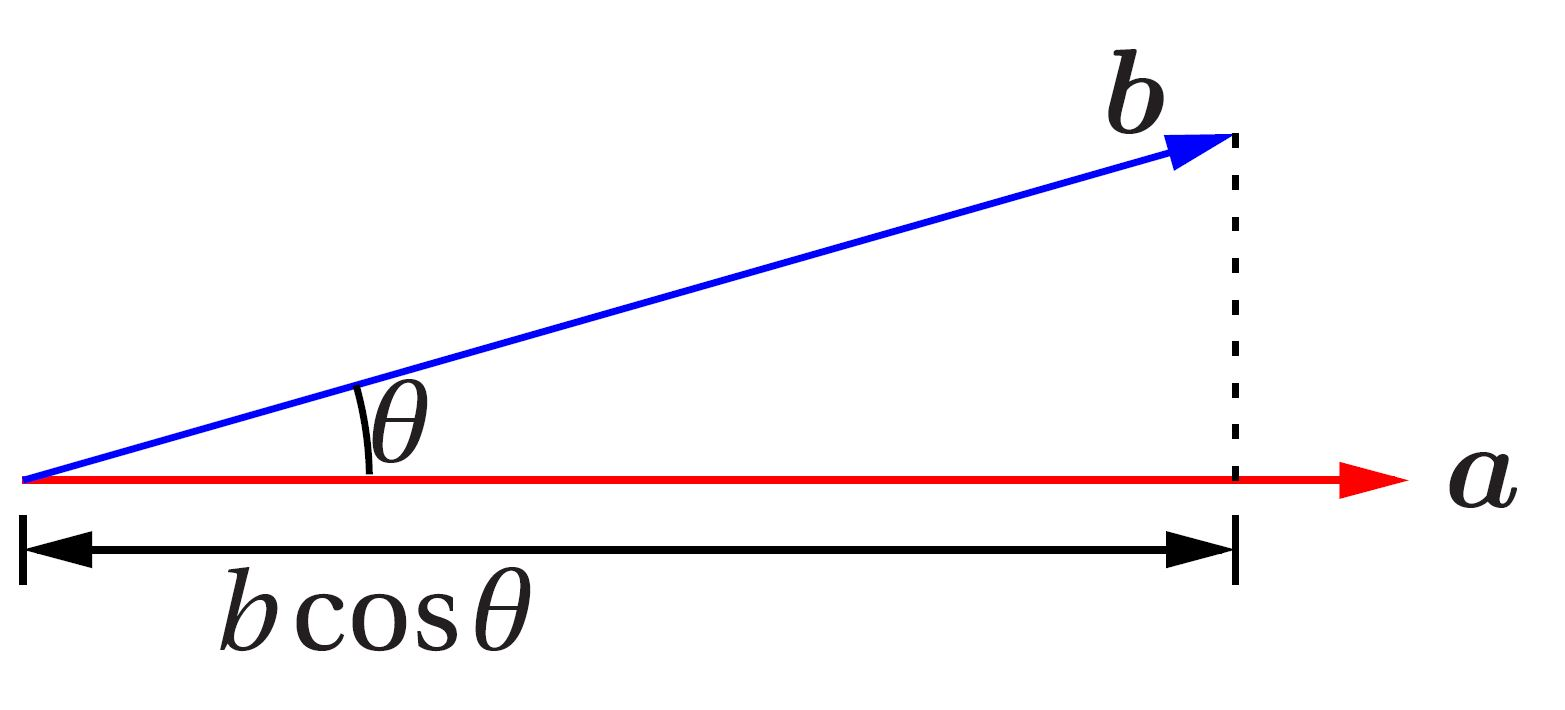
\includegraphics[width=0.34\textwidth]{images/fig1-4}
  \caption{내적의 의미}
  \label{fig:dotproduct}
\end{wrapfigure}

같은 두개의 벡터의 내적을 제곱으로 정의하고, 그 결과는 벡터의 크기의 제곱과 같으므로, 벡터의 크기는 내적의 제곱근으로 나타낼 수 있다.
\[
  \vb{a}^2 \equiv \vb{a} \vdot \vb{a} = a^2 \Longleftrightarrow a = \sqrt{\vb{a}^2} = \sqrt{\vb{a} \vdot \vb{a}}
\]

기본 단위 벡터는 크기가 1이고 서로 수직인 벡터이므로 다음의 관계식을 만족한다.
\[
  \vb{e}_i \vdot \vb{e}_j  = \delta_{ij}
\]
여기서 $\delta_{ij}$는 크로네커 델타(Kronecker delta)라 불리며 다음과 같이 정의되어 있다.
\[
  \sigma_{ij} = \begin{cases}
    i & (i = j)    \\
    0 & (i \neq j)
  \end{cases}
\]
이 성질을 이용하면 벡터의 내적을 성분으로 나타낼 수 있다.
\begin{align*}
  \vb{a} \vdot \vb{b} & = (a_x \vb{e}_x + a_y \vb{e}_y + a_z \vb{e}_z) \vdot (b_x \vb{e}_x + b_y \vb{e}_y + b_z \vb{e}_z) \\
                      & = a_x b_x + a_y b_y + a_z b_z                                                                     \\
                      & = \sum_i{a_i b_i}
\end{align*}
즉, 벡터의 내적은 각 성분의 곱을 합한 것과 같다.

벡터를 열벡터로 나타내면 내적은 $\vb{a}^t$($\vb{a}$의 전치 행렬\footnote{$n \cp m$의 행렬 $\vb{A} = (A_{ij})$의 전치 행렬은 $n \cp m$의 행렬 $\vb{A}^t = (A_{ji})$을 가리킨다. 즉, 대각 성분에 대해서 성분을 뒤집은 행렬이다.}
\[
  \vb{a} \vdot \vb{b} = \begin{pmatrix}
    a_x & a_y & a_z
  \end{pmatrix} \begin{pmatrix}
    b_x \\
    b_y \\
    b_z
  \end{pmatrix} = a_x b_x + a_y b_y + a_z b_z
\]
특히, 어떤 벡터와 기본 단위 벡터의 내적은 해당 축 방향의 성분
\[
  a_i = \vb{a} \vdot \vb{e}_i
\]
와 같다.

성분을 알 수 있는 두 벡터가 있다면
\[
  \cos{\theta} = \frac{\vb{a} \vdot \vb{b}}{ab} = \frac{a_x b_x + a_y b_y + a_z b_z}{ab}
\]
의 방법으로 두 벡터의 사잇각을 계산할 수 있다.

\subsection{외적}
두 벡터 $\vb{a}$, $\vb{b}$에 대해서 외적(outer product, cross product)은 $\vb{a} \cp \vb{b}$라고 쓴다. 외적의 결과는 또다른 벡터이므로 벡터곱(vector product)이라고도 불리며, 외적은 방향과 크기를 갖는다. 외적의 방향은 그림 \placeholder와 같이 $\vb{a}$에서 $\vb{b}$로 사잇각이 작은 쪽으로 회전시켰을 때 오른나사가 진행하는 방향\footnote{$\vb{a}$에서 $\vb{b}$로 한손으로 오른손으로 감쌌을 때 엄지가 향하는 방향이라고도 표현한다.}으로 정의한다. 외적의 크기는
\[
  \norm{\vb{a} \cp \vb{b}} = ab \sin{\theta}
\]
로 정의되고, 이는 $\vb{a}$와 $\vb{b}$로 그려지는 평행사변형(그림 \placeholder의 초록색 부분)의 넓이와 같다.

벡터의 외적에 대해서는 분배 법칙이 성립하지만 일반적으로 결합 법칙은 성립하지 않는다.

\[
  (\vb{a} \cp \vb{b}) \cp \neq \vb{a} \cp (\vb{b} \cp \vb{c})
\]
\[
  \vb{a} \cp (\vb{b} + \vb{c}) = \vb{a} \cp \vb{b} + \vb{a} \cp \vb{c}
\]

한편, 교환 법칙은 성립하지 않으나 벡터의 순서가 뒤바뀌면 사잇각이 그대로 이므로 크기가 같고 방향이 반대인 벡터가 되며, 평행한 두 벡터의 외적은 사잇각이 0이므로 0이 된다.
\[
  \vb{a} \cp \vb{b} = - \vb{b} \cp \vb{a}, \quad \vb{a} \cp \vb{a} = 0
\]

데카르트 좌표계는 오른손 좌표계\footnote{$x$축에서 $y$축으로 오른손을 감아 쥐었을 때 $z$축의 방향이 엄지손가락의 방향이 되는 좌표계}이기 때문에, 기본 단위 벡터 둘을 순서대로 외적하면 나머지 기본 단위 벡터가 얻어진다.
\[
  \vb{e}_x \cp \vb{e}_y = \vb{e}_z, \quad \vb{e}_y \cp \vb{e}_z = \vb{e}_x, \quad \vb{e}_z \cp \vb{e}_x = \vb{e}_y
\]
곱의 순서가 바뀌면 $-$부호가 붙는다. 또한 같은 단위 벡터들의 외적은 0이다. 이로부터 벡터의 외적을 성분으로 나타내면 다음과 같다.
\begin{align*}
  \vb{a} \cp \vb{b} & = (a_x \vb{e}_x + a_y \vb{e}_y + a_z \vb{e}_z) \cp (b_x \vb{e}_x + b_y \vb{e}_y + b_z \vb{e}_z \\
                    & = (a_y b_z - a_z b_y)\vb{e}_x + (a_z b_x - a_x b_z)\vb{e}_y + (a_x b_y - a_y b_x)\vb{e}_z
\end{align*}
외적은 성분으로 나타내면 $x, y, z$의 순서대로 반복적으로 성분과 기본 단위 벡터가 나타난다는 규칙성이 있으나 표현이 번잡하다. 행렬식의 계산에 익숙하다면 다음과 같은 표기가 더 간단할 수 있다.
\[
  \vb{a} \cp \vb{b} = \begin{vmatrix}
    \vb{e}_x & \vb{e}_y & \vb{e}_z \\
    a_x      & a_y      & a_z      \\
    b_x      & b_y      & b_z
  \end{vmatrix} = \begin{vmatrix}
    a_y & a_z \\
    b_y & b_z
  \end{vmatrix} \vb{e}_x - \begin{vmatrix}
    a_x & a_z \\
    b_x & b_z
  \end{vmatrix} \vb{e}_y + \begin{vmatrix}
    a_x & a_y \\
    b_x & b_y
  \end{vmatrix} \vb{e}_z = \begin{pmatrix}
    a_y b_z - a_z b_y \\
    a_z b_x - a_x b_z \\
    a_x b_y - a_y b_x
  \end{pmatrix}
\]

\subsubsection{스칼라 삼중곱}
다음과 같은 형태의 벡터곱을 스칼라 삼중곱(scalar triple product)이라 한다.
\[
  \vb{a} \vdot (\vb{b} \cp \vb{c}) = \begin{vmatrix}
    a_x & a_y & a_z \\
    b_x & b_y & b_z \\
    c_z & c_y & c_z
  \end{vmatrix}
\]
스칼라 삼중곱은 다음과 같이 순서대로 곱의 순서를 바꿀 수 있다.
\[
  \vb{a} \vdot (\vb{b} \cp \vb{c}) = \vb{b} \vdot (\vb{c} \cp \vb{a}) = \vb{c} \vdot (\vb{b} \cp \vb{a})
\]
또한 스칼라 삼중곱은 세 벡터를 세 변으로 가지는 평행육면체의 부피와 같다.

\subsubsection{벡터 삼중곱}
다음과 같은 형태의 곱을 벡터 삼중곱(vector triple product)이라 한다.
\[
  \vb{a} \cp (\vb{b} \cp \vb{c})
\]
벡터 삼중곱의 결과는 벡터이며 다음 등식을 만족한다.
\[
  \vb{a} \cp (\vb{b} \cp \vb{c}) = (\vb{a} \vdot \vb{c}) \vb{b} - (\vb{a} \vdot \vb{b}) \vb{c}
\]
이로부터 $\vb{a} \cp (\vb{b} \cp \vb{c})$는 $\vb{b}$와 $\vb{c}$를 포함하는 평면 속에 존재함을 알 수 있다.

\end{document}
